\renewcommand{\stage}{From inference to control}

\begin{frame}{Let's deal with control now}
We observe position, but braking also depends on velocity.
\begin{center}\begin{tikzpicture}[every node/.style={font=\small,align=center}]
\path[use as bounding box] (-2,-2.6) rectangle (8,1.8);
\foreach \x in {0,6}{
\draw[black!45] (\x-1.9,-.5)--(\x+1.9,-.5);
\draw[fill=blue!10,draw=blue,thick] (\x-.5,-.3) rectangle (\x+.5,.3);
\draw[dashed] (\x,-.5)--(\x,-1);\node at (\x,-1.2) {Same position $x$};}
\draw[arr,blue] (.6,.5)--(1.9,.5) node[midway,above]{velocity};
\draw[arr,pink,visible on=<2->] (-.6,-.1)--(-1.9,-.1) node[midway,above]{force};
\draw[arr,blue] (5.4,.5)--(4.1,.5) node[midway,above]{velocity};
\draw[arr,pink,visible on=<2->] (6.6,-.1)--(7.9,-.1) node[midway,above]{force};
\node[visible on=<3->] (hist) at (0,-2.3) {Position history};
\node[visible on=<3->] (bel) at (6,-2.3) {Distribution of position and velocity};
\draw[arr,visible on=<3->] (hist)--node[above]{filter}(bel);
\end{tikzpicture}\end{center}

\end{frame}

\begin{frame}{QMDP assumes future states will be observed}
Our current belief $b$ is a distribution over position and velocity.
\begin{center}\begin{tikzpicture}[x=1cm,y=.9cm,font=\small]
\path[use as bounding box] (0,-.65) rectangle (12.4,3.5);
\node[lab] at (2.8,3.3) {Belief planning};
\node[obj] (b) at (2.8,2.6) {$b$};
\foreach \x/\n/\i in {1.4/l/1,4.2/r/2}{\node[circle,draw,inner sep=2pt] (\n) at (\x,1.6) {};\draw[arr] (b)--node[above,lab]{$a_{\i}$}(\n);}
\foreach \x/\n in {.6/l,2.2/l,3.4/r,5/r}{\draw[arr] (\n)--(\x,.6);\draw[arr,black!40] (\x,.6)--(\x-.3,.1);\draw[arr,black!40] (\x,.6)--(\x+.3,.1);}
\node[lab] at (2.8,-.4) {Branch on future observations};
\begin{scope}[visible on=<2->]
\node[lab] at (9.3,3.3) {QMDP approximation};
\node[obj] (bq) at (7.4,2.55) {$b$};
\node[obj] (aq) at (9.05,2.55) {$a$};
\draw[arr] (bq)--(aq);
\draw[arr] (aq)--(10.7,2.55)--(10.7,1.65);
\node[lab] at (9.3,1.15) {Assume the state is revealed\\after action $a$};
\draw[arr] (9.3,.55)--(9.3,.05);
\node[lab] at (9.3,-.4) {Use fully observed control};
\end{scope}
\end{tikzpicture}\end{center}
\uncover<3->{\[
Q_{\mathrm{QMDP}}(b,a)=
\underbrace{\E_{X\sim b}}_{\text{uncertainty now}}
\big[\underbrace{Q^*_{\mathrm{fully\ observed}}(X,a)}_{\text{act, then observe the state}}\big].
\]}
\uncover<3->{Choose the action with the largest average return. No future observation tree.}
\src{QMDP uses the Q-values of the fully observed Markov decision process. It can miss the value of actions that gather information.}
\end{frame}

\begin{frame}{Using the particle filter to choose actions}
{\small Model fitting: earlier paper. State inference: particle filter. Now we add planning.}
\begin{center}\begin{tikzpicture}
\node[inner sep=0,anchor=south west] (pipeline) at (0,0) {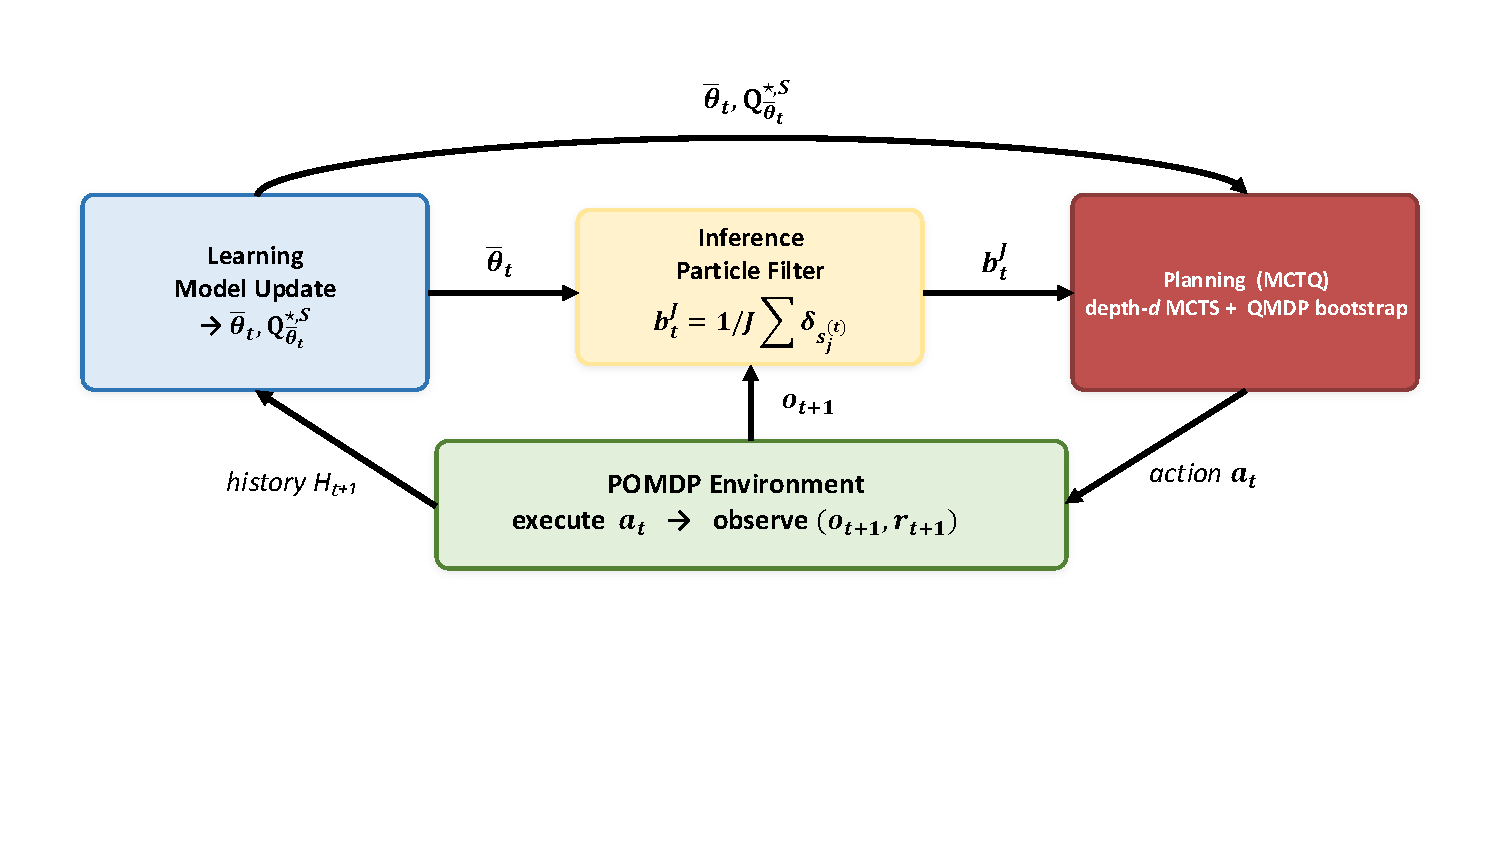
\includegraphics[height=4.1cm]{control-pipeline.pdf}};
\begin{scope}[x={(pipeline.south east)},y={(pipeline.north west)}]
% Keep the original illustration; reset only the small planning label in vector text.
\definecolor{planningred}{HTML}{BD4F4A}
\fill[planningred] (.741,.43) rectangle (.988,.66);
\node[text=white,font=\fontsize{8.5}{10}\selectfont,align=center] at (.866,.545)
 {Planning (MCTQ)\\depth-$d$ MCTS\\+ QMDP bootstrap};
\end{scope}
\end{tikzpicture}\end{center}
{\small $\bar\theta$: fitted model. $b^J$: particle belief. $H_t$: observed history.}\par\smallskip
\uncover<2->{\gap\small Experiments: learned dynamics, actor and critic; state rollouts with belief-tree depth $d=0$.}
\src{Tan and Xu, NeurIPS 2026. Theoretical planner: belief tree with QMDP at its leaves.}
\end{frame}

\begin{frame}{MuJoCo with partially observed states}
\begin{columns}[c,onlytextwidth]
\column{.64\textwidth}
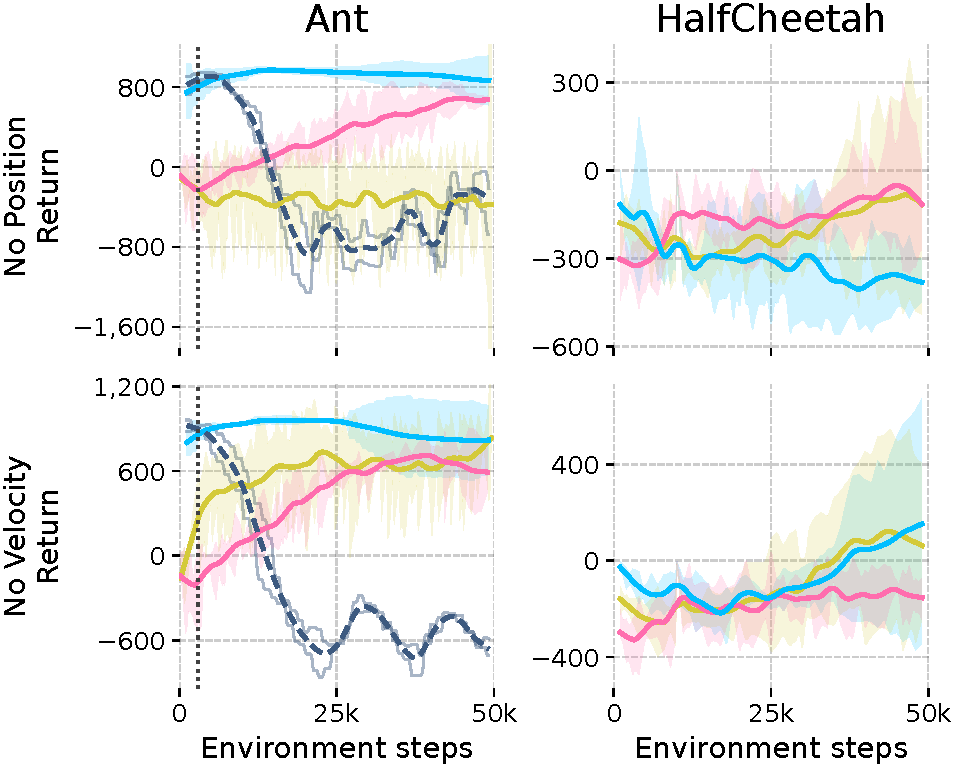
\includegraphics[width=\linewidth,height=6.0cm,keepaspectratio]{control-mujoco-selected.pdf}
\column{.34\textwidth}
{\small Dynamics are learned online.}
\par\medskip
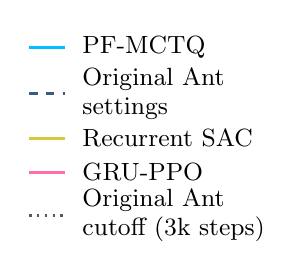
\begin{tikzpicture}[font=\fontsize{9}{10.5}\selectfont,x=1cm,y=1cm]
\definecolor{pfcurve}{HTML}{00BEFF}\definecolor{oldpfcurve}{HTML}{3D5A80}\definecolor{saccurve}{HTML}{D4CA3A}\definecolor{ppocurve}{HTML}{FF6DAE}
\draw[pfcurve,very thick] (0,0)--(.45,0);\node[anchor=west] at (.55,0){PF-MCTQ};
\draw[oldpfcurve,thick,dashed] (0,-.58)--(.45,-.58);\node[anchor=west,align=left] at (.55,-.58){Original Ant\\settings};
\draw[saccurve,very thick] (0,-1.15)--(.45,-1.15);\node[anchor=west] at (.55,-1.15){Recurrent SAC};
\draw[ppocurve,very thick] (0,-1.58)--(.45,-1.58);\node[anchor=west] at (.55,-1.58){GRU-PPO};
\draw[black!65,thick,dotted] (0,-2.13)--(.45,-2.13);\node[anchor=west,align=left] at (.55,-2.13){Original Ant\\cutoff (3k steps)};
\end{tikzpicture}
\par\medskip
{\small Revised Ant settings prevent the later collapse.}
\uncover<2->{\par\medskip\small No gain on HalfCheetah with positions hidden.}
\end{columns}
\src{Tan and Xu, Fig. 3 (selected panels). Training return, 95\% $t$ bands. Five seeds; Ant PF-MCTQ: three revised, two original.}
\end{frame}

\begin{frame}{Two themes from my dissertation}
\begin{columns}[T,onlytextwidth]
\column{.47\textwidth}
{\Large\color{blue}Learning to act}\gap
The maximum target removes dependence on a changing policy.
\pause
\column{.47\textwidth}
{\Large\color{green}Fitting a model}\gap
Fixed parents and corrected weights give a differentiable likelihood estimate.
\end{columns}
\uncover<3->{\gap In partially observed control, we estimate the state and then choose an action.}
\end{frame}

\begin{frame}{Thank you everyone!}
\medskip
{\small To my advisors Yuting and Giles, \\
\qquad Enric for being on my committee,\\
and my favorite collaborators \\
\qquad Wei, Chinmaya, Haimo, Zhihan, Joey, Will, Junu, Kunyang, Pingbang, \\
\qquad Ziping, Sharan, Ambuj, and Ed.}
\end{frame}
